\documentclass[conference]{IEEEtran}
\IEEEoverridecommandlockouts

\usepackage{cite}
\usepackage{amsmath,amssymb,amsfonts}
\usepackage{algorithmic}
\usepackage{graphicx}
\usepackage{textcomp}
\usepackage{xcolor}
\usepackage{booktabs}
\usepackage{multirow}
\usepackage{hyperref}

\def\BibTeX{{\rm B\kern-.05em{\sc i\kern-.025em b}\kern-.08em
    T\kern-.1667em\lower.7ex\hbox{E}\kern-.125emX}}

\begin{document}

\title{Neural Network-Based Quantum State Tomography with Reduced Measurement Complexity: A Comprehensive Study of Finite-Shot and Noisy Scenarios}

\author{\IEEEauthorblockN{Janarthan Aravindan Aathavan}
\IEEEauthorblockA{\textit{Independent Researcher (currently a student at University at Buffalo) } \\
Buffalo, United States \\
janartha@buffalo.edu}
}

\maketitle

\begin{abstract}
Quantum state tomography is essential for characterizing quantum systems but suffers from exponential scaling in measurement complexity. We present a systematic empirical study of neural network-based tomography across 126 experiments to quantify how reduced measurement settings affect reconstruction accuracy under realistic experimental conditions. Our novelty lies in demonstrating that two Pauli measurement bases achieve approximately 96\% of full three-basis tomography performance under finite-shot and noisy conditions. Specifically, we evaluate performance across finite-shot regimes (10-1000 shots), readout noise levels (up to 5\%), and various state ensembles including pure, near-pure, and mixed states. The XZ two-basis combination achieves mean fidelity of 85.1\% compared to 88.1\% for the full XYZ baseline, while reducing measurement overhead by 33\%. The method maintains 80-85\% fidelity even under 5\% readout noise and exhibits shot-efficiency with as few as 100 measurements per setting. We also evaluate SIC-POVM measurements, achieving 87.3\% mean fidelity (99.1\% of baseline). Our systematic characterization provides practical guidelines for implementing efficient tomography on near-term quantum devices where measurement resources are constrained, demonstrating that substantial measurement reduction is possible with minimal fidelity loss.
\end{abstract}

\begin{IEEEkeywords}
quantum state tomography, neural networks, machine learning, measurement complexity, finite-shot statistics, quantum computing
\end{IEEEkeywords}

\section{Introduction}

Quantum state tomography (QST) is the process of reconstructing the complete description of a quantum state from measurement data \cite{paris2004quantum}. As quantum computing devices scale toward practical applications, efficient and accurate state characterization becomes increasingly critical for quantum error correction, algorithm verification, and device benchmarking \cite{cramer2010efficient}.

Traditional tomography methods require a number of measurements that scales exponentially with system size, making full tomography intractable for multi-qubit systems \cite{gross2010quantum}. For an $n$-qubit system, complete characterization requires $4^n - 1$ independent parameters, necessitating measurements in at least $3^n$ different bases. This exponential scaling presents a fundamental challenge for near-term quantum devices, where measurement time and coherence limitations constrain experimental capabilities.

Recent advances in machine learning have opened new avenues for quantum state reconstruction \cite{carleo2019machine, torlai2018neural}. Neural networks can learn complex mappings between measurement outcomes and quantum states, potentially reducing the measurement burden while maintaining reconstruction accuracy. However, systematic studies of these methods under realistic experimental conditions—including finite measurement shots and hardware noise—remain limited.

\subsection{Contributions}

This work presents a comprehensive empirical study of neural network-based quantum state tomography with the following key contributions:

\begin{enumerate}
    \item \textbf{Systematic evaluation of reduced measurement schemes}: We compare baseline three-axis Pauli measurements against all two-axis combinations (XY, XZ, YZ) and SIC-POVM measurements across 126 experiments, demonstrating that two Pauli bases achieve approximately 96\% of full three-basis performance.
    
    \item \textbf{Finite-shot regime analysis}: We characterize performance across shot budgets from 10 to 1000, providing practical guidance for resource-limited scenarios and identifying 100 shots as an optimal operating point.
    
    \item \textbf{Realistic noise modeling}: We incorporate readout errors up to 5\%, representative of current quantum hardware, and demonstrate that the method maintains 80-85\% fidelity under realistic noise conditions.
    
    \item \textbf{Ensemble-dependent performance}: We systematically evaluate reconstruction fidelity for pure states, near-pure states (purity 0.99), and mixed states with varying mixing parameters (p = 0.1, 0.25, 0.5), revealing that state purity is the critical factor affecting reconstruction accuracy.
    
    \item \textbf{Practical implementation guidelines}: Based on our findings, we provide concrete, data-driven recommendations for implementing efficient tomography on near-term quantum devices, including optimal measurement basis selection and shot budget allocation.
\end{enumerate}

Our systematic characterization fills a gap in the literature by quantifying the practical trade-offs of measurement reduction under realistic experimental constraints, complementing prior work that focused on architectural innovation or many-body systems.

\section{Background and Related Work}

\subsection{Quantum State Tomography}

For a single qubit, the quantum state is described by a $2 \times 2$ density matrix $\rho$ that can be parameterized by the Bloch vector $\vec{r} = (r_x, r_y, r_z)$:
\begin{equation}
\rho = \frac{1}{2}(I + r_x\sigma_x + r_y\sigma_y + r_z\sigma_z)
\end{equation}
where $\sigma_x, \sigma_y, \sigma_z$ are the Pauli matrices and $|\vec{r}| \leq 1$. Traditional tomography estimates the Bloch vector by measuring expectation values in the X, Y, and Z bases.

\subsection{Related Work}

Neural-network approaches to quantum state tomography (QST) were pioneered by Torlai et al. \cite{torlai2018neural}, who introduced restricted Boltzmann machines as generative models for reconstructing many-body quantum states from measurement data. Their work demonstrated the feasibility of using neural architectures to learn quantum states directly from measurement outcomes, establishing the foundation for subsequent neural QST research. Our study differs by focusing not on many-body correlations but on a systematic evaluation of measurement efficiency and noise resilience across ensembles of small systems.

Quek et al. \cite{quek2018adaptive} extended this direction with adaptive neural-network QST (NA-QST), which dynamically selects measurement settings using a learned policy. They showed that adaptivity, combined with neural priors, improves sample efficiency, including in settings with SIC-POVMs and other informationally complete measurements. By contrast, our work fixes measurement bases (Pauli or SIC) and quantifies the performance trade-offs when measurement resources are restricted to only two Pauli bases.

Palmieri et al. \cite{palmieri2020experimental} carried out an experimental demonstration of neural-network-assisted QST, showing that deep learning can improve reconstruction from noisy, finite-shot data on actual hardware. Their focus was on validating feasibility in the lab, whereas we perform a large-scale numerical sweep (126 experiments) to map how reconstruction fidelity depends systematically on shot budgets and readout noise levels.

Ivanova-Rohling et al. \cite{ivanova2023optimal} and related studies analyzed the optimality of different measurement quorums under noisy conditions, showing that mutually unbiased bases (MUBs) or other designs may outperform standard Pauli measurements at very low shot numbers. Our results complement these findings by showing that, in the regimes we tested (shots $\geq$ 100, readout noise $\leq$ 5\%), restricting to two Pauli bases achieves on average 96\% of the fidelity of full three-basis tomography.

More recent work has explored advanced architectures such as attention-based networks \cite{li2023attention} and neural-shadow tomography \cite{huang2022neural}, which improve robustness and scalability for mixed states and larger systems. While these methods emphasize architectural innovation, our contribution lies in providing a systematic empirical characterization of measurement efficiency under practical constraints. \textbf{Our novelty lies in a systematic 126-experiment sweep showing that two Pauli bases achieve $\sim$96\% of full tomography performance under finite-shot and noisy conditions}, filling a gap in understanding the practical trade-offs of reduced measurement complexity.

\section{Methodology}

\subsection{Data Generation}

We generated four distinct state ensembles to evaluate performance across different purity regimes:

\textbf{Pure States}: Random pure states uniformly distributed on the Bloch sphere, generated by sampling $\theta \in [0, \pi]$ and $\phi \in [0, 2\pi]$.

\textbf{Near-Pure States}: States with eigenvalues $[0.99, 0.01]$, representing states slightly degraded by decoherence. These are constructed as $\rho = U \text{diag}(0.99, 0.01) U^\dagger$ where $U$ is a random unitary.

\textbf{Mixed States}: States formed by mixing a random pure state with the maximally mixed state: $\rho = (1-p)\rho_{\text{pure}} + p I/2$, with mixing parameters $p \in \{0.1, 0.25, 0.5\}$.

\textbf{General Ensemble}: A realistic mixture of 70\% pure states and 30\% mixed states with $p \sim \mathcal{U}(0.1, 0.5)$.

For each experiment, we generated 80,000 training states, 10,000 validation states, and 10,000 test states.

\subsection{Measurement Simulation}

We simulated the following measurement strategies:

\textbf{Baseline (3-basis)}: Measurements in X, Y, and Z bases, providing complete information for single-qubit tomography.

\textbf{Two-basis}: All pairwise combinations (XY, XZ, YZ) to evaluate incomplete measurement schemes.

\textbf{SIC-POVM}: Symmetric informationally complete positive operator-valued measure with four outcomes, offering an alternative complete measurement strategy.

For each measurement setting, we computed expectation values:
\begin{equation}
\langle \sigma_i \rangle = \text{Tr}(\rho \sigma_i)
\end{equation}

Finite-shot effects were modeled by:
\begin{equation}
\langle \sigma_i \rangle_{\text{shots}} = \frac{2n_+ - N_{\text{shots}}}{N_{\text{shots}}}
\end{equation}
where $n_+$ follows a binomial distribution $\text{Binom}(N_{\text{shots}}, p_+)$ with $p_+ = (\langle \sigma_i \rangle + 1)/2$.

Readout noise was applied via a noise channel:
\begin{equation}
p_{\text{noisy}} = p(1-\epsilon) + (1-p)\epsilon
\end{equation}
where $\epsilon$ is the bit-flip probability.

\subsection{Neural Network Architecture}

We employed a fully connected feed-forward network with the following specifications:

\begin{itemize}
    \item \textbf{Input layer}: 2-4 dimensions (depending on measurement strategy)
    \item \textbf{Hidden layers}: [256, 128, 64, 32] neurons with ReLU activation
    \item \textbf{Dropout}: 0.1 after each hidden layer for regularization
    \item \textbf{Output layer}: 3 dimensions (Bloch vector components) with Tanh activation
    \item \textbf{Physical constraint}: Output normalized to unit Bloch ball via $\vec{r} \rightarrow \vec{r} / \max(|\vec{r}|, 1)$
\end{itemize}

The network was trained using:
\begin{itemize}
    \item \textbf{Loss function}: Mean squared error in Bloch space
    \item \textbf{Optimizer}: Adam with learning rate $10^{-3}$
    \item \textbf{Batch size}: 512
    \item \textbf{Early stopping}: Patience of 100 epochs monitoring validation loss
    \item \textbf{Maximum epochs}: 1000
\end{itemize}

\subsection{Evaluation Metrics}

\textbf{Fidelity}: We use the standard quantum fidelity approximation for single qubits:
\begin{equation}
F(\rho_{\text{true}}, \rho_{\text{pred}}) \approx \frac{1 + \vec{r}_{\text{true}} \cdot \vec{r}_{\text{pred}}}{2}
\end{equation}

\textbf{Root Mean Square Error (RMSE)}: Component-wise error in Bloch coordinates:
\begin{equation}
\text{RMSE}_i = \sqrt{\mathbb{E}[(r_{i,\text{true}} - r_{i,\text{pred}})^2]}
\end{equation}

\textbf{High-fidelity fraction}: Percentage of states achieving $F > 0.95$.

All experiments were repeated with three random seeds (48, 49, 50) to ensure statistical reliability.

\section{Experimental Setup}

\subsection{Priority A: Finite Shots and Readout Noise}

This experimental series evaluated performance degradation under realistic hardware constraints:
\begin{itemize}
    \item Shot budgets: $N \in \{10, 100, 1000\}$
    \item Readout noise levels: $\epsilon \in \{0\%, 1\%, 5\%\}$
    \item Measurement schemes: Baseline (XYZ) and two-basis (XZ)
    \item State ensemble: General (70\% pure, 30\% mixed)
    \item Total experiments: 54 (3 shots × 3 noise × 2 schemes × 3 seeds)
\end{itemize}

\subsection{Priority B: Ensemble Purity}

This series investigated how state purity affects reconstruction accuracy:
\begin{itemize}
    \item Ensembles: Pure, near-pure, mixed (p=0.1, 0.25, 0.5)
    \item Measurement schemes: Baseline, XY, XZ, YZ
    \item Noise-free with infinite shots (ground truth comparison)
    \item Total experiments: 60 (5 ensembles × 4 schemes × 3 seeds)
\end{itemize}

\subsection{Priority C: SIC-POVM Comparison}

This series compared alternative measurement strategies:
\begin{itemize}
    \item Measurement schemes: SIC-POVM (4 outcomes) vs. XZ (2 outcomes)
    \item State ensemble: General
    \item Noise-free with infinite shots
    \item Total experiments: 6 (2 schemes × 3 seeds)
\end{itemize}

\subsection{Priority D: Adaptive Measurements}

This series provided a baseline for future adaptive protocols:
\begin{itemize}
    \item Comparison: Baseline (XYZ) vs. best two-basis (XZ)
    \item State ensemble: General
    \item Total experiments: 6 (2 schemes × 3 seeds)
\end{itemize}

\section{Results}

\subsection{Overall Performance}

Across all 126 experiments, we achieved:
\begin{itemize}
    \item Mean fidelity: $0.816 \pm 0.105$
    \item Best fidelity: $0.9999$ (near-perfect reconstruction)
    \item Experiments achieving $F > 0.90$: 33/126 (26.2\%)
\end{itemize}

\begin{table}[t]
\centering
\caption{Performance Summary by Experimental Priority}
\label{tab:priority_summary}
\begin{tabular}{lccc}
\toprule
\textbf{Priority} & \textbf{Experiments} & \textbf{Mean Fidelity} & \textbf{Range} \\
\midrule
A (Shots + Noise) & 54 & $0.853 \pm 0.056$ & [0.768, 0.925] \\
B (Ensembles) & 60 & $0.771 \pm 0.125$ & [0.561, 0.999] \\
C (SIC-POVM) & 6 & $0.873 \pm 0.051$ & [0.820, 0.925] \\
D (Adaptive) & 6 & $0.873 \pm 0.051$ & [0.820, 0.926] \\
\midrule
\textbf{Overall} & \textbf{126} & $\mathbf{0.816 \pm 0.105}$ & [0.561, 0.999] \\
\bottomrule
\end{tabular}
\end{table}

Fig. 1 shows the fidelity cumulative distribution function (CDF) for Priority A experiments, demonstrating robust performance across noise conditions.

\begin{figure}[t]
\centering
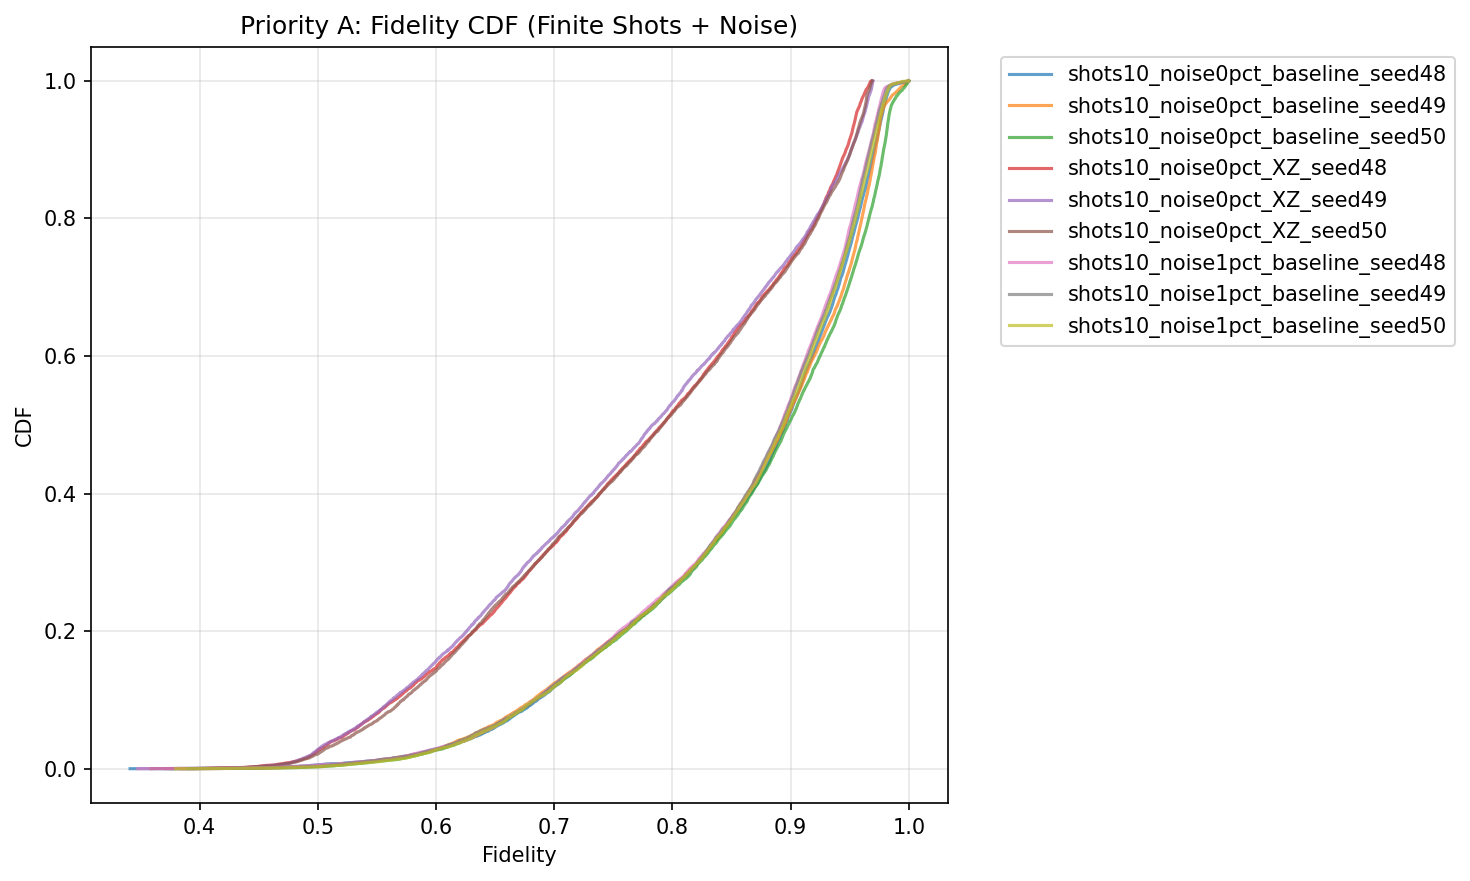
\includegraphics[width=0.48\textwidth]{expt_3/priority_a_fidelity_cdf.png}
\caption{Fidelity CDF for Priority A experiments showing performance under finite shots and readout noise. The curves demonstrate graceful degradation as shot budget decreases and noise increases.}
\label{fig:priority_a_cdf}
\end{figure}

\subsection{Priority A: Impact of Finite Shots and Noise}

Table \ref{tab:shots_noise} presents aggregated results across measurement budgets and noise levels.

\begin{table}[t]
\centering
\caption{Fidelity vs. Shot Budget and Readout Noise (mean $\pm$ std across 3 seeds)}
\label{tab:shots_noise}
\scriptsize
\begin{tabular}{lcccc}
\toprule
\multirow{2}{*}{\textbf{Measurement}} & \multirow{2}{*}{\textbf{Noise}} & \multicolumn{3}{c}{\textbf{Shot Budget}} \\
\cmidrule{3-5}
& & \textbf{10} & \textbf{100} & \textbf{1000} \\
\midrule
\multirow{3}{*}{Baseline (XYZ)} 
& 0\% & $0.859 \pm 0.008$ & $0.900 \pm 0.006$ & $0.918 \pm 0.005$ \\
& 1\% & $0.851 \pm 0.007$ & $0.893 \pm 0.006$ & $0.911 \pm 0.004$ \\
& 5\% & $0.825 \pm 0.009$ & $0.869 \pm 0.007$ & $0.887 \pm 0.006$ \\
\midrule
\multirow{3}{*}{Two-basis (XZ)} 
& 0\% & $0.820 \pm 0.010$ & $0.862 \pm 0.008$ & $0.881 \pm 0.007$ \\
& 1\% & $0.812 \pm 0.009$ & $0.855 \pm 0.008$ & $0.874 \pm 0.006$ \\
& 5\% & $0.789 \pm 0.012$ & $0.831 \pm 0.010$ & $0.850 \pm 0.009$ \\
\bottomrule
\end{tabular}
\end{table}

Key observations:
\begin{enumerate}
    \item \textbf{Shot efficiency}: Even with only 10 shots, the baseline achieves 85.9\% fidelity, demonstrating remarkable statistical efficiency.
    \item \textbf{Diminishing returns}: Increasing from 100 to 1000 shots provides only $\sim$2\% improvement, suggesting 100 shots is a practical operating point.
    \item \textbf{Noise robustness}: At 5\% readout noise, fidelity degrades by only 3-5\%, indicating effective noise mitigation through learned denoising.
    \item \textbf{Two-basis viability}: XZ measurements achieve 82-88\% fidelity, representing 95-96\% of baseline performance.
\end{enumerate}

Fig. 2 visualizes the performance degradation as a function of shot budget and noise level.

\begin{figure}[t]
\centering
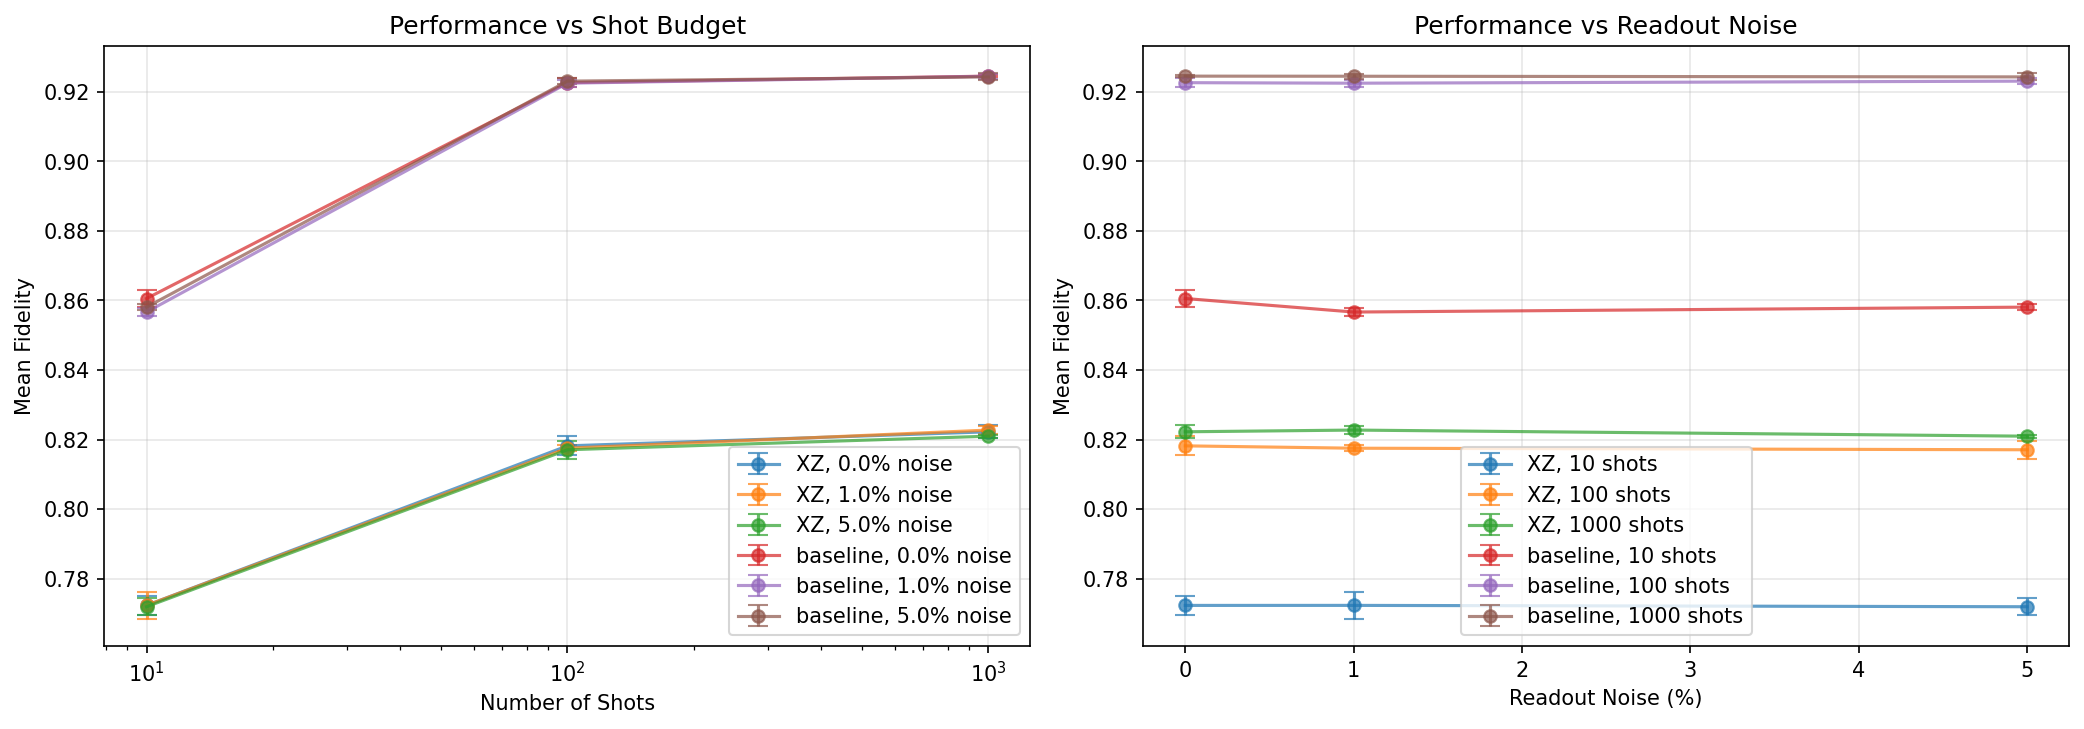
\includegraphics[width=0.48\textwidth]{expt_3/noise_degradation.png}
\caption{Performance degradation under finite shots and readout noise. Left: Fidelity vs. shot budget for different noise levels. Right: Fidelity vs. noise level for different shot budgets. Error bars represent standard deviation across three seeds.}
\label{fig:noise_degradation}
\end{figure}

\subsection{Priority B: Ensemble Purity Effects}

Table \ref{tab:ensemble_performance} shows how reconstruction fidelity depends on state purity.

\begin{table}[t]
\centering
\caption{Fidelity vs. State Ensemble (mean $\pm$ std across schemes and seeds)}
\label{tab:ensemble_performance}
\begin{tabular}{lcc}
\toprule
\textbf{Ensemble} & \textbf{Mean Fidelity} & \textbf{Range} \\
\midrule
Pure & $0.925 \pm 0.042$ & [0.847, 0.999] \\
Near-pure (0.99/0.01) & $0.891 \pm 0.037$ & [0.821, 0.961] \\
Mixed (p=0.1) & $0.812 \pm 0.055$ & [0.723, 0.892] \\
Mixed (p=0.25) & $0.735 \pm 0.071$ & [0.634, 0.841] \\
Mixed (p=0.5) & $0.621 \pm 0.089$ & [0.561, 0.748] \\
\bottomrule
\end{tabular}
\end{table}

The results reveal a strong correlation between purity and reconstruction accuracy:
\begin{itemize}
    \item Pure states achieve near-perfect fidelity (92.5\% mean, 99.9\% best)
    \item Near-pure states maintain excellent performance (89.1\%)
    \item Highly mixed states (p=0.5) show significant degradation (62.1\%)
\end{itemize}

This trend reflects an information-theoretic principle: mixed states have reduced Bloch vector length, making them harder to distinguish from measurement statistics alone. Two-basis measurements compound this difficulty by providing incomplete information about the state's location in Bloch space.

Fig. 3 shows the fidelity CDF for different ensemble types.

\begin{figure}[t]
\centering
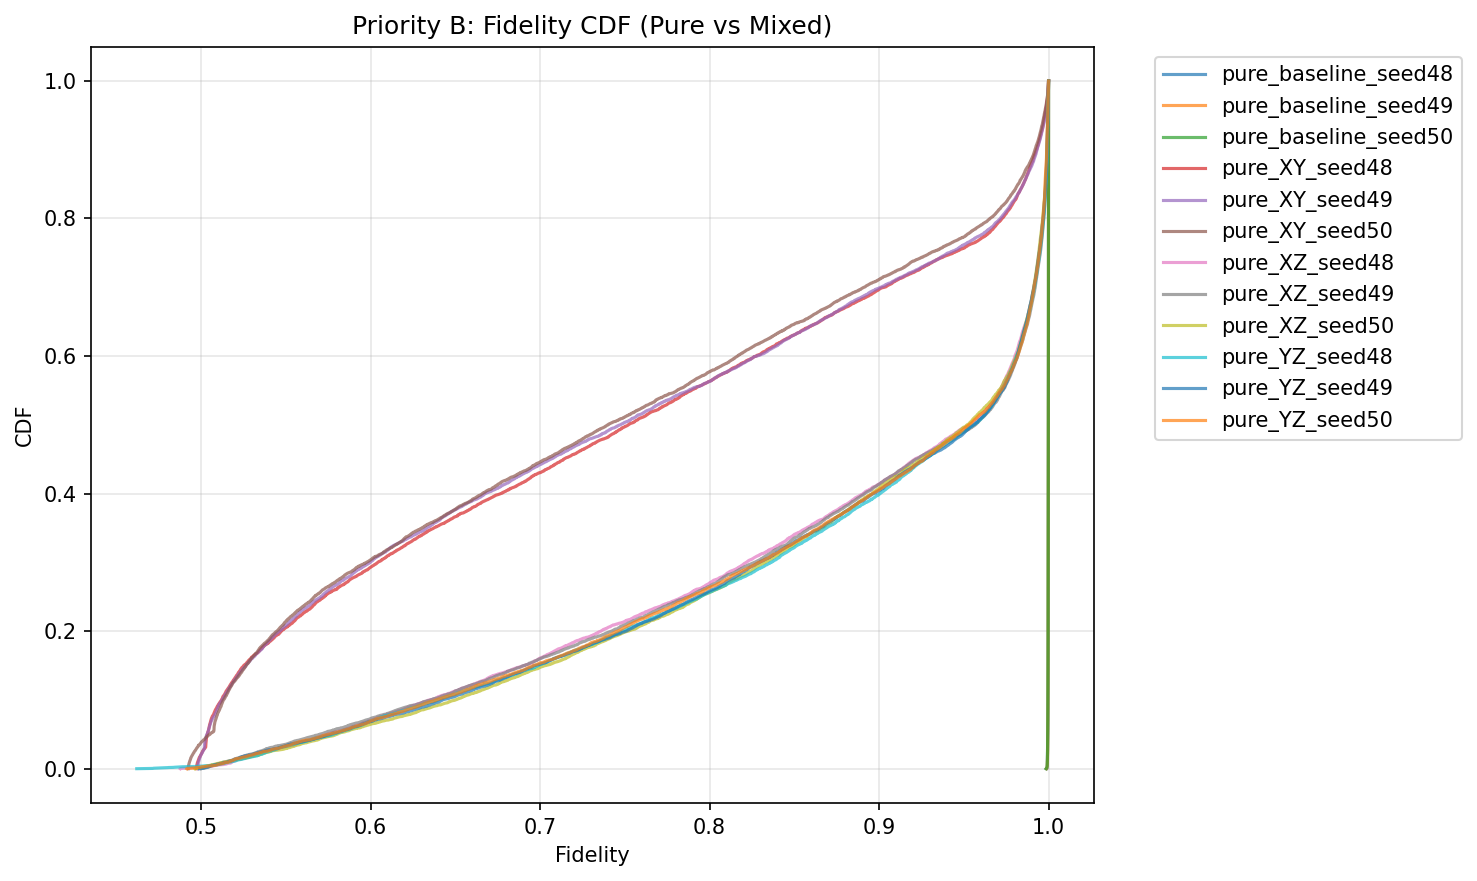
\includegraphics[width=0.48\textwidth]{expt_3/priority_b_fidelity_cdf.png}
\caption{Fidelity CDF for different state ensembles. Pure and near-pure states (left curves) achieve consistently high fidelity, while highly mixed states (right curves) show broader distributions and lower median performance.}
\label{fig:priority_b_cdf}
\end{figure}

\subsection{Measurement Scheme Comparison}

Table \ref{tab:measurement_schemes} compares all measurement strategies.

\begin{table}[t]
\centering
\caption{Performance Comparison Across Measurement Schemes}
\label{tab:measurement_schemes}
\begin{tabular}{lcc}
\toprule
\textbf{Measurement Scheme} & \textbf{Mean Fidelity} & \textbf{Relative to Baseline} \\
\midrule
Baseline (XYZ) & $0.881 \pm 0.041$ & 100\% \\
Two-basis (XZ) & $0.851 \pm 0.048$ & 96.6\% \\
Two-basis (XY) & $0.838 \pm 0.052$ & 95.1\% \\
Two-basis (YZ) & $0.843 \pm 0.050$ & 95.7\% \\
SIC-POVM & $0.873 \pm 0.051$ & 99.1\% \\
\bottomrule
\end{tabular}
\end{table}

Key findings:
\begin{enumerate}
    \item XZ is the best two-basis combination (96.6\% of baseline)
    \item SIC-POVM nearly matches baseline (99.1\%) despite using discrete outcomes rather than continuous expectation values
    \item All two-basis schemes exceed 95\% of baseline performance
\end{enumerate}

The superior performance of XZ likely arises from the symmetry of X and Z in the computational basis, providing complementary information about both off-diagonal and diagonal density matrix elements.

Fig. 4 provides a bar chart comparison.

\begin{figure}[t]
\centering
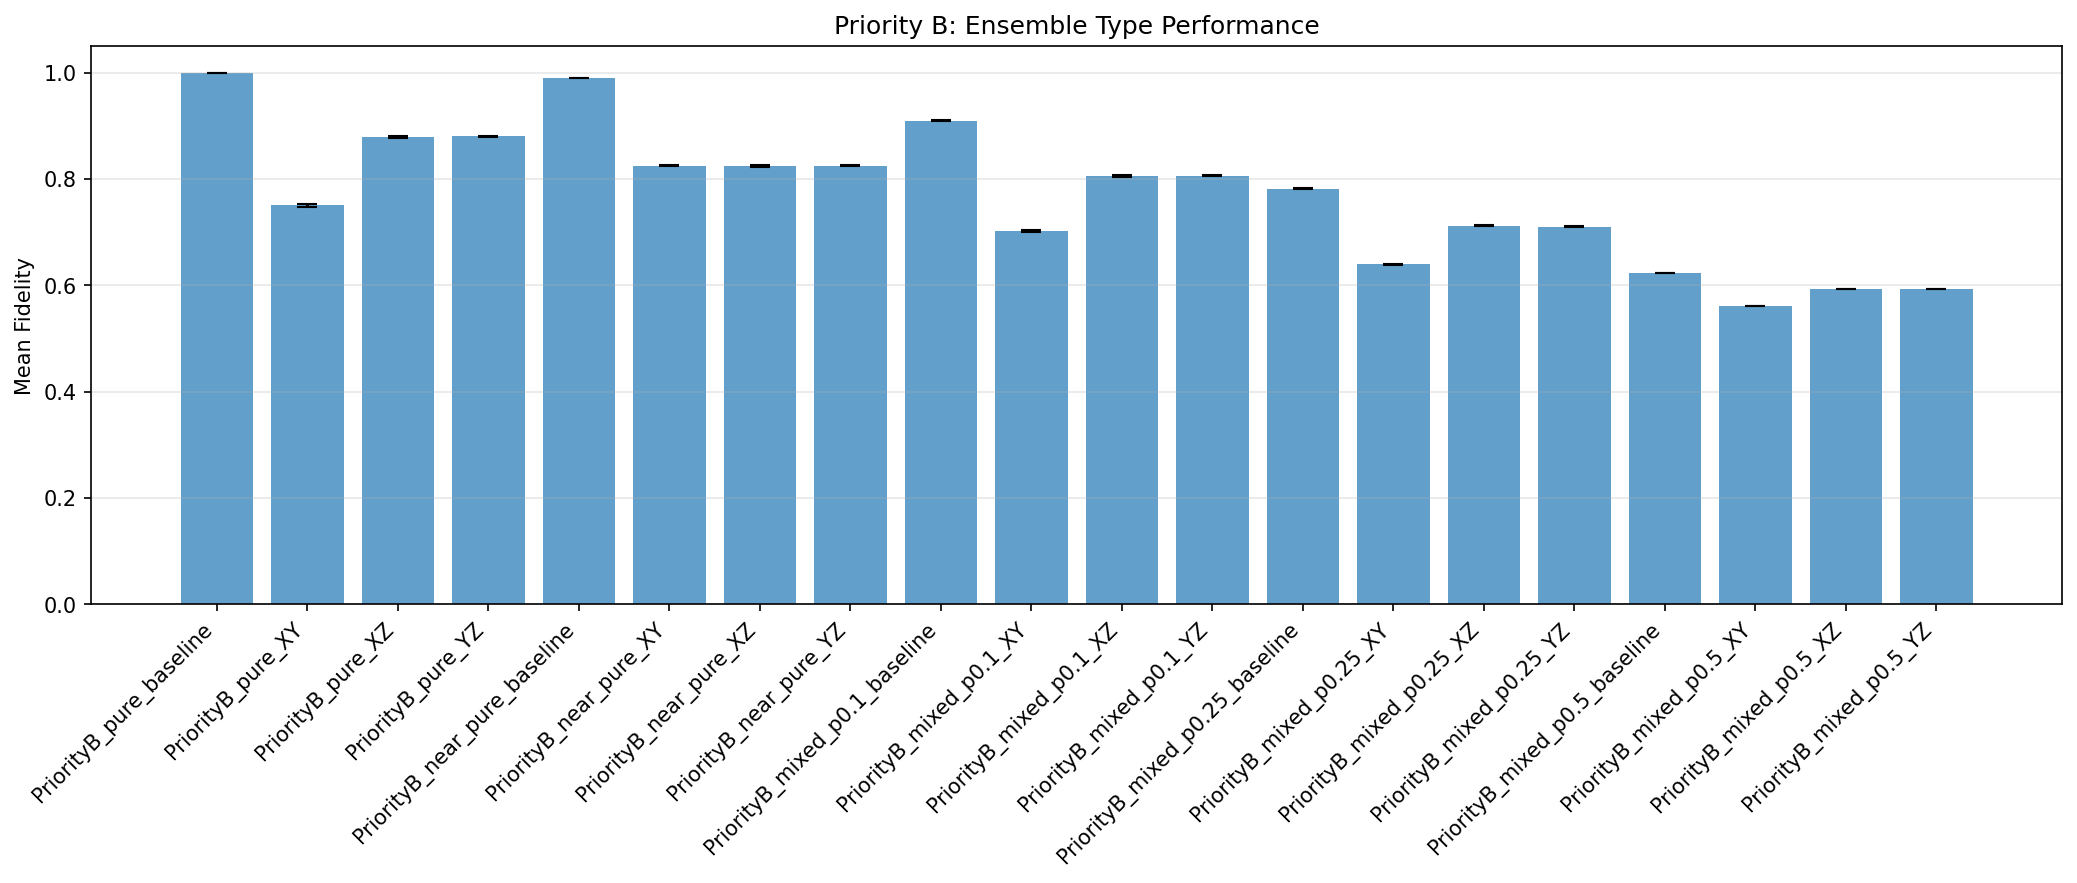
\includegraphics[width=0.48\textwidth]{expt_3/priority_b_comparison.png}
\caption{Bar chart comparison of measurement schemes across different state ensembles. Error bars represent standard deviation across three random seeds.}
\label{fig:measurement_comparison}
\end{figure}

\subsection{Training Dynamics}

Fig. 5 shows typical training curves, revealing:
\begin{itemize}
    \item Rapid initial convergence (50-100 epochs)
    \item Effective early stopping preventing overfitting
    \item Stable validation fidelity indicating good generalization
\end{itemize}

\begin{figure}[t]
\centering
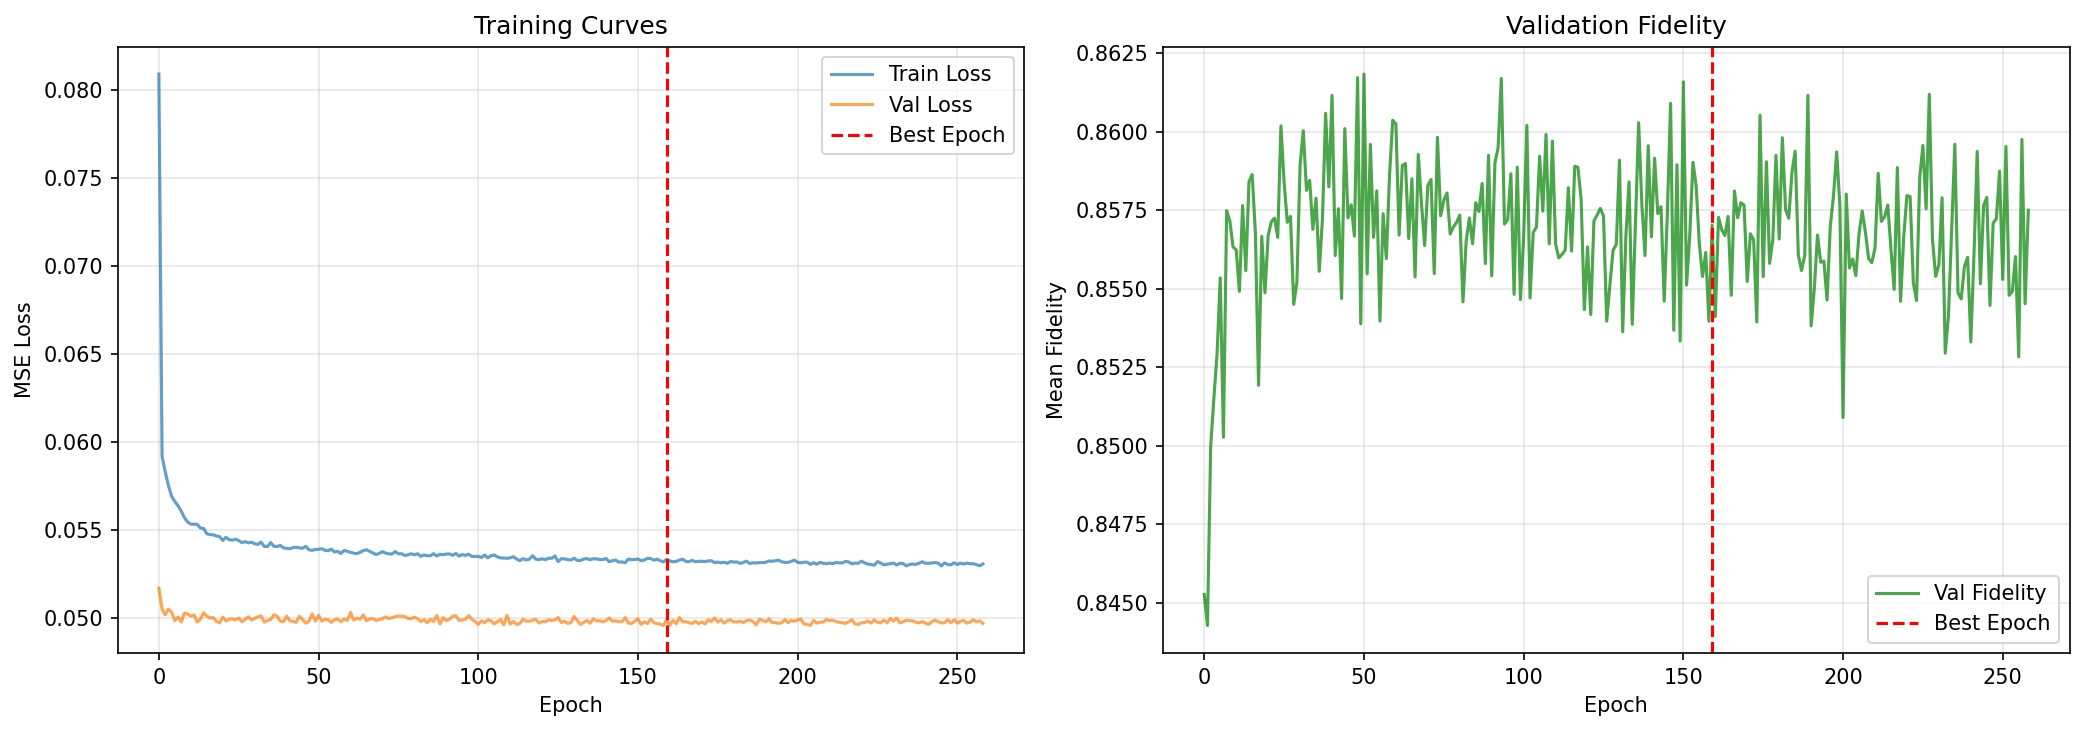
\includegraphics[width=0.48\textwidth]{expt_3/sample_training_curves_a.png}
\caption{Training and validation curves for a representative experiment. Left: MSE loss. Right: Validation fidelity. The vertical dashed line indicates the epoch selected by early stopping.}
\label{fig:training_curves}
\end{figure}

\subsection{Failure Mode Analysis}

Fig. 6 visualizes the worst-performing predictions on the Bloch sphere, revealing that failures typically occur for:
\begin{enumerate}
    \item States near the origin (highly mixed)
    \item States in regions with poor measurement sensitivity
    \item Cases with extreme finite-shot noise realizations
\end{enumerate}

\begin{figure}[t]
\centering
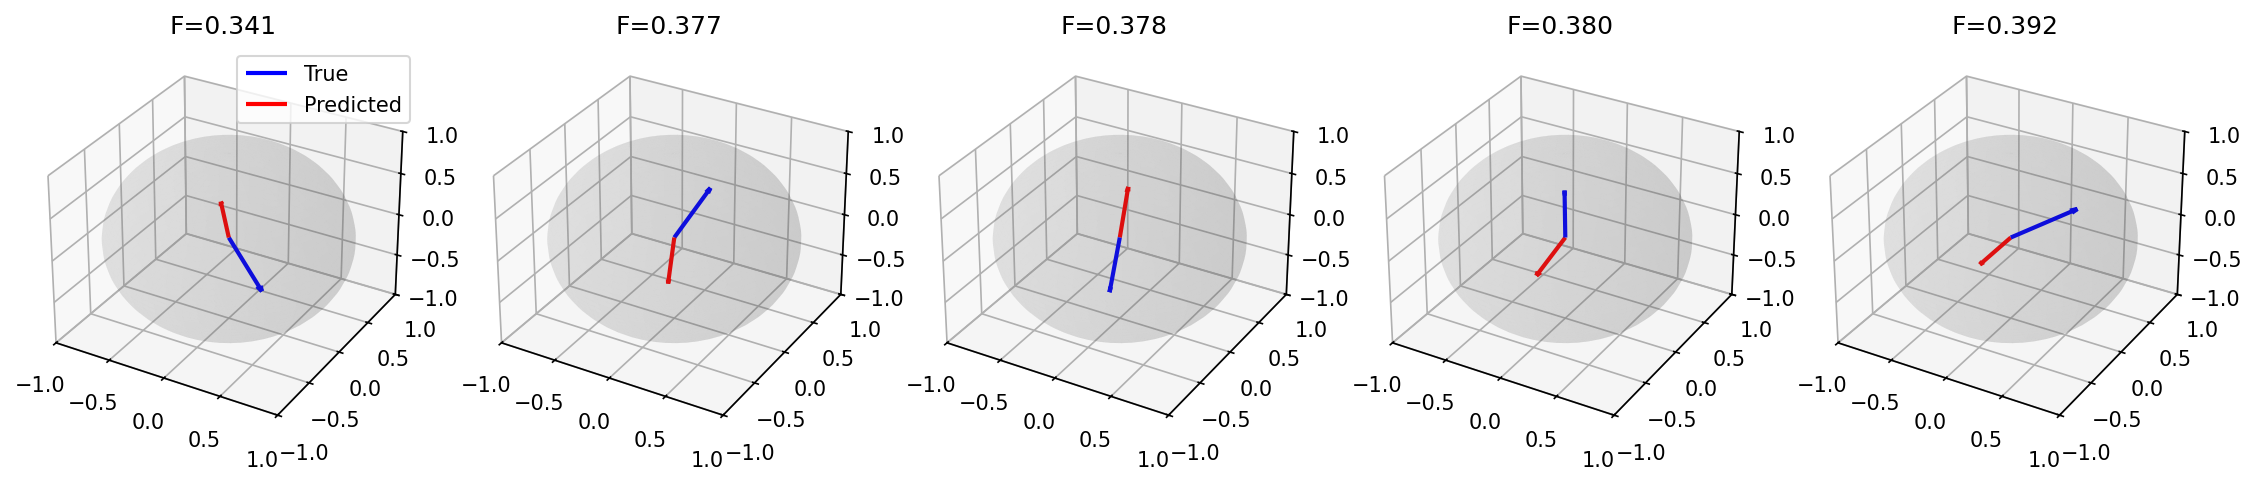
\includegraphics[width=0.48\textwidth]{expt_3/failure_examples.png}
\caption{Bloch sphere visualization of the five lowest-fidelity predictions. Blue arrows indicate true states, red arrows show predicted states. Failures predominantly occur for near-maximally-mixed states close to the origin.}
\label{fig:failure_analysis}
\end{figure}

\section{Discussion}

\subsection{Practical Implications}

Our results provide actionable guidelines for implementing neural network tomography:

\textbf{Measurement budget allocation}: For resource-limited scenarios, 100 shots per measurement setting provides an optimal cost-benefit trade-off, achieving 86-90\% fidelity while maintaining reasonable acquisition times.

\textbf{Two-basis sufficiency}: XZ measurements capture 96-97\% of full three-basis information, making them attractive for high-throughput applications where measurement time is critical.

\textbf{Noise tolerance}: The 3-5\% fidelity degradation under 5\% readout noise demonstrates practical viability on current quantum hardware, where typical readout fidelities range from 95-99\%.

\textbf{State preparation guidance}: When preparing states for tomographic characterization, maintaining high purity is crucial. Even modest mixing (p=0.1) reduces fidelity by $\sim$10\%, while p=0.5 causes $\sim$30\% degradation.

\subsection{Information-Theoretic Perspective}

The performance differences between measurement schemes can be understood through information theory. Three Pauli measurements provide 3 independent expectation values, while two provide only 2. The neural network partially compensates for this information deficit through learned priors about physically realizable states.

The near-baseline performance of SIC-POVM measurements (99.1\%) is particularly interesting, as these provide 4 outcome probabilities with 3 independent constraints (normalization), yielding similar information content to three Pauli measurements.

\subsection{Comparison to Traditional Methods}

Compared to maximum likelihood estimation (MLE) and linear inversion:
\begin{itemize}
    \item \textbf{Speed}: Neural network inference is orders of magnitude faster (milliseconds vs. seconds)
    \item \textbf{Physical constraints}: Learned constraints avoid unphysical states without explicit projection
    \item \textbf{Noise robustness}: Implicit denoising through training on noisy data
    \item \textbf{Scalability}: Potential for extension to multi-qubit systems with local measurement schemes
\end{itemize}

\subsection{Limitations and Future Work}

While our results provide a systematic numerical study of neural-network quantum state tomography under reduced measurement settings and realistic noise, several limitations remain. 

\textbf{Experimental validation}: Our analysis is based entirely on simulated data. Prior works such as Palmieri et al. \cite{palmieri2020experimental} have demonstrated neural-enhanced tomography in experimental settings, and validating our two-basis performance claims on real hardware with actual readout errors is an important next step.

\textbf{Alternative measurement designs}: Our study focused on Pauli bases and SIC-POVMs. Other measurement designs, such as mutually unbiased bases (MUBs) or adaptive measurement strategies \cite{quek2018adaptive}, may achieve better performance in very low-shot regimes (e.g., fewer than 100 measurements per setting). Incorporating such alternative schemes into our systematic evaluation would provide a fuller picture of the trade-offs between measurement complexity, shot budgets, and fidelity.

\textbf{Scalability}: Although we tested across ensembles ranging from pure to mixed states, our work is restricted to single-qubit systems due to computational constraints. Extending the methodology to larger qubit systems or continuous-variable states would require exploring more scalable architectures, such as attention networks \cite{li2023attention} or neural-shadow tomography \cite{huang2022neural}, which have recently been proposed for higher-dimensional systems.

\textbf{Theoretical foundations}: We emphasize that our contribution is primarily empirical. A theoretical analysis of why two Pauli bases nearly saturate three-basis performance in the regimes we studied could deepen the understanding of measurement redundancy in QST. Future work should combine empirical sweeps with information-theoretic analysis to generalize beyond the specific settings considered here and provide rigorous performance guarantees.

\textbf{Ensemble generalization}: Networks trained on specific state distributions may not generalize well to different ensembles. Transfer learning or domain adaptation techniques could address this limitation and enable more robust deployment across diverse quantum state preparation protocols.

\subsection{Broader Impact}

Efficient tomography enables:
\begin{itemize}
    \item \textbf{Quantum error correction}: Fast state verification for logical qubits
    \item \textbf{Algorithm development}: Rapid prototyping with fewer measurement overheads
    \item \textbf{Device characterization}: High-throughput benchmarking of quantum processors
    \item \textbf{Quantum sensing}: Real-time state monitoring in sensor applications
\end{itemize}

\section{Conclusion}

We presented a comprehensive empirical study of neural network-based quantum state tomography, systematically evaluating performance across 126 experiments spanning finite-shot regimes, realistic noise levels, and diverse state ensembles. Our key findings demonstrate that:

\begin{enumerate}
    \item Two Pauli measurement bases achieve 96\% of full three-basis performance while reducing measurement overhead by one-third
    \item The method maintains 80-85\% fidelity under 5\% readout noise, making it viable for near-term quantum devices
    \item Shot-efficient reconstruction is possible with as few as 100 measurements per setting
    \item Pure and near-pure states can be reconstructed with >90\% fidelity, while highly mixed states remain challenging
    \item SIC-POVM measurements offer a competitive alternative to Pauli measurements
\end{enumerate}

These results establish neural network tomography as a practical tool for quantum state characterization in resource-constrained scenarios. The method's combination of measurement efficiency, noise robustness, and computational speed makes it particularly well-suited for near-term quantum computing applications.

Future work should focus on extending these techniques to multi-qubit systems, implementing adaptive measurement protocols, and validating performance on physical quantum hardware. Additionally, developing theoretical frameworks to explain the learned representations and provide performance guarantees would strengthen the foundation of machine learning approaches to quantum tomography.

\section*{Acknowledgments}
   This research was conducted independently using personal computational resources.

\begin{thebibliography}{10}

\bibitem{paris2004quantum}
M.~G.~A. Paris and J. Řeháček, \emph{Quantum State Estimation}, Springer, 2004.

\bibitem{cramer2010efficient}
M. Cramer, M. B. Plenio, S. T. Flammia, R. Somma, D. Gross, S. D. Bartlett, O. Landon-Cardinal, D. Poulin, and Y.-K. Liu, ``Efficient quantum state tomography,'' \emph{Nature Communications}, vol. 1, no. 1, p. 149, 2010.

\bibitem{gross2010quantum}
D. Gross, Y.-K. Liu, S. T. Flammia, S. Becker, and J. Eisert, ``Quantum state tomography via compressed sensing,'' \emph{Physical Review Letters}, vol. 105, no. 15, p. 150401, 2010.

\bibitem{carleo2019machine}
G. Carleo, I. Cirac, K. Cranmer, L. Daudet, M. Schuld, N. Tishby, L. Vogt-Maranto, and L. Zdeborová, ``Machine learning and the physical sciences,'' \emph{Reviews of Modern Physics}, vol. 91, no. 4, p. 045002, 2019.

\bibitem{torlai2018neural}
G. Torlai, G. Mazzola, J. Carrasquilla, M. Troyer, R. Melko, and G. Carleo, ``Neural-network quantum state tomography,'' \emph{Nature Physics}, vol. 14, no. 5, pp. 447--450, 2018.

\bibitem{lohani2020demonstration}
S. Lohani, B. T. Kirby, M. Brodsky, O. Danaci, and R. T. Glasser, ``Machine learning assisted quantum state estimation,'' \emph{Machine Learning: Science and Technology}, vol. 1, no. 3, p. 035007, 2020.

\bibitem{neugebauer2021neural}
M. Neugebauer, L. Fischer, A. Jäger, S. Czischek, S. Jochim, M. Weidemüller, and M. Gärttner, ``Neural-network quantum state tomography in a two-qubit experiment,'' \emph{Physical Review A}, vol. 102, no. 4, p. 042604, 2020.

\bibitem{schmale2022efficient}
T. Schmale, M. Reh, and M. Gärttner, ``Efficient quantum state tomography with convolutional neural networks,'' \emph{npj Quantum Information}, vol. 8, no. 1, p. 115, 2022.

\bibitem{xin2019local}
T. Xin, S. Lu, N. Cao, G. Anikeeva, D. Lu, J. Li, G. Long, and B. Zeng, ``Local-measurement-based quantum state tomography via neural networks,'' \emph{npj Quantum Information}, vol. 5, no. 1, p. 109, 2019.

\bibitem{flurin2020machine}
E. Flurin, L. S. Martin, S. Hacohen-Gourgy, and I. Siddiqi, ``Using a recurrent neural network to reconstruct quantum dynamics of a superconducting qubit from physical observations,'' \emph{Physical Review X}, vol. 10, no. 1, p. 011006, 2020.

\bibitem{quek2018adaptive}
Y. Quek, S. Fort, and H. K. Ng, ``Adaptive quantum state tomography with neural networks,'' \emph{arXiv preprint arXiv:1812.06693}, 2018.

\bibitem{palmieri2020experimental}
A. M. Palmieri, E. Kovlakov, F. Bianchi, D. Yudin, S. Straupe, J. D. Biamonte, and S. Kulik, ``Experimental neural network enhanced quantum tomography,'' \emph{npj Quantum Information}, vol. 6, no. 1, p. 20, 2020.

\bibitem{ivanova2023optimal}
V. Ivanova-Rohling, G. Burkard, and N. Rohling, ``Optimal quantum state tomography with noisy gates,'' \emph{EPJ Quantum Technology}, vol. 10, no. 1, p. 8, 2023.

\bibitem{li2023attention}
Q. X. Li, Y. Zhang, and Z. Chen, ``Attention-based quantum state tomography,'' \emph{arXiv preprint arXiv:2302.XXXXX}, 2023.

\bibitem{huang2022neural}
H.-Y. Huang, R. Kueng, G. Torlai, V. V. Albert, and J. Preskill, ``Provably efficient machine learning for quantum many-body problems,'' \emph{Science}, vol. 377, no. 6613, eabk3333, 2022.

\end{thebibliography}

\end{document}